本章主要介绍拉格朗日力学和哈密顿力学, 它们都是经典力学的重新表述, 与牛顿力学等价, 前者由拉格朗日于 1788 创立, 后者由哈密顿于 1833 年创立. 重新表述经典力学这件事本身不是最重要的, 最重要的是这两种框架非常强力, 因而被广泛使用于后续的物理中. 可以说, 想要学物理, 就必须先了解它们.

牛顿力学以 $ F=ma $ 及受力分析的方法为公理, 虽然``力''这个概念易于理解, 但实际操作起来麻烦, 在对比较复杂的系统作受力分析时要处处小心. 实际上, 力 (force) 这个概念是多余的, 我们完全可以绕过它来建立力学 (mechanics).

\section{拉格朗日力学}
在拉格朗日力学中, 真正重要的概念只有拉格朗日量和最小作用量原理, 其余所有东西都可以由它们推出.

考虑 $ \mathbb{R}^n $ 中若干个质点组成的系统, 其所有 (在约束下) 可能状态的全体构成了\textbf{位形空间} (configuration space). 能用来唯一地表示位形空间中的点的一组参数 $ q=(q^1,\dots,q^k) $ 叫做\textbf{广义坐标}, 其中的 $ k $ 叫做系统的\textbf{自由度}. 

系统状态随时间的演化构成了位形空间中的一条曲线 $ \gamma(t) $, 它的广义坐标 $ q(t)=(q_1(t),\dots,q_k(t)) $ 关于时间 $ t $ 的导数 $ \dot{q}(t) $ 叫做\textbf{广义速度}.
\begin{definition}[拉格朗日量]
    给定势能 $ V $, 则其对应的{\bf 拉格朗日量} (Lagrangian) 为函数 $ L(q,\dot{q},t):=T-V $, 其中 $ q $ 是广义坐标, $ \dot{q} $ 是广义速度, $ T $ 是动能, $ V $ 是势能.
\end{definition}
本书只考虑最简单的情况: 质量为 $ m $ 的质点的{\bf 动能}
\[ T=\frac{1}{2}m\dot{q}^2, \] 
对于多个质点构成的系统, 其动能为所有质点的动能之和; {\bf 势能} $ V $ 是位形空间上的函数. 此时 $ L $ 不显含时间变量 $ t $, 可将其记为 $ L(q,\dot{q}) $.

\begin{definition}[作用量]
    给定 $ [t_1,t_2]\subset\mathbb{R} $, 则{\bf 作用量} (action) 为泛函
    \[ S[q] :=\int_{t_1}^{t_2}L(q(t),\dot{q}(t),t)\,\mathrm{d}t.\]
\end{definition}

对于泛函 $ I(q) $, 固定 $ q=q_0 $, 若有 $ I(q_0+h)-I(q_0)=A(h)+R(q_0,h) $, 其中 $ A $ 关于 $ h $ 是线性的, 且 $ R(q_0,h)=o(h) $, 则称 $ I $ 是可微的, 称 $ A $ 为 $ I $ 在 $ q_0 $ 处的微分 (Fr\'{e}chet 导数). 泛函的微分又叫做变分, 记作 $ \delta I $.

\begin{axiom}[最小作用量原理]
    固定 $ q(t_1) $ 和 $ q(t_2) $, 则时间段 $ [t_1,t_2] $ 上的真实物理过程是满足 $ \delta S=0 $ 的 $ q(t) $.
\end{axiom}
\begin{remark}
    最小作用量原理也叫哈密顿原理. 
\end{remark}
\begin{theorem}[拉格朗日方程]
    最小作用量原理等价于{\bf 拉格朗日方程}
    \[ \frac{\partial L}{\partial q}-\frac{\mathrm{d}}{\mathrm{d}t}\frac{\partial L}{\partial\dot{q}}=0. \]
\end{theorem}
\begin{proof}
对于 $ S $, 有
\begin{align*}
    S[q+h]-S[q] &= \int_{t_1}^{t_2}\left[ L(q+h,\dot{q}+\dot{h},t)-L(q,\dot{q},t) \right]\mathrm{d}t\\ 
    &=\int_{t_1}^{t_2}\left[ \frac{\partial L}{\partial q}h+\frac{\partial L}{\partial\dot{q}}\dot{h} \right]\mathrm{d}t+o(h).
\end{align*}
由于 $ q(t_1) $ 和 $ q(t_2) $ 被固定了, 有 $ h(t_1)=h(t_2)=0 $. 由分部积分可得
\begin{align*}
    \int_{t_1}^{t_2}\frac{\partial L}{\partial\dot{q}}\dot{h}\,\mathrm{d}t &= \left.h\frac{\partial L}{\partial\dot{q}}\right|_{t_1}^{t_2}-\int_{t_1}^{t_2}h\frac{\mathrm{d}}{\mathrm{d}t}\left( \frac{\partial L}{\partial\dot{q}} \right)\mathrm{d}t\\ 
    &=-\int_{t_1}^{t_2}h\frac{\mathrm{d}}{\mathrm{d}t}\left( \frac{\partial L}{\partial\dot{q}} \right)\mathrm{d}t.
\end{align*}
综上有
\[ S[q+h]-S[q]=\int_{t_1}^{t_2}\left[ \frac{\partial L}{\partial q}-\frac{\mathrm{d}}{\mathrm{d}t}\frac{\partial L}{\partial\dot{q}} \right] h\,\mathrm{d}t + o(h). \]

根据定义, $ S $ 在 $ q $ 处的变分为
\[ \delta S[q](h) = \int_{t_1}^{t_2}\left[ \frac{\partial L}{\partial q}-\frac{\mathrm{d}}{\mathrm{d}t}\frac{\partial L}{\partial\dot{q}} \right] h\,\mathrm{d}t, \]
因此 $ \delta S=0 $ 等价于 
\[ \frac{\partial L}{\partial q}-\frac{\mathrm{d}}{\mathrm{d}t}\frac{\partial L}{\partial\dot{q}}=0. \qedhere\]
\end{proof}

若定义广义动量 $p$ 和广义力 $F$ 为
\[ p:=\frac{\partial L}{\partial\dot{q}},\quad F:=\frac{\partial L}{\partial q}, \] 
则拉格朗日方程可表达为 $ F=\dot{p} $, 与 $F=ma$ 形式一致. 在牛顿力学中, 我们先做受力分析, 然后解 $ F=ma $, 从而得到质点的运动轨迹; 在拉格朗日力学中, 我们先写出拉格朗日量, 然后解拉格朗日方程, 从而得到 $ q(t) $.

与牛顿力学相比, 拉格朗日力学的优势在于不需要做繁琐的受力分析, 更适合处理复杂系统. 我们可以从下面这个经典例子中一窥拉格朗日力学的优雅.

\begin{example}[双摆]
    如图 \ref{double pendulum} 所示, 假设两小球为质点, 连接他们的杆是无质量刚体. 
    \begin{figure}[H]
        \centering
        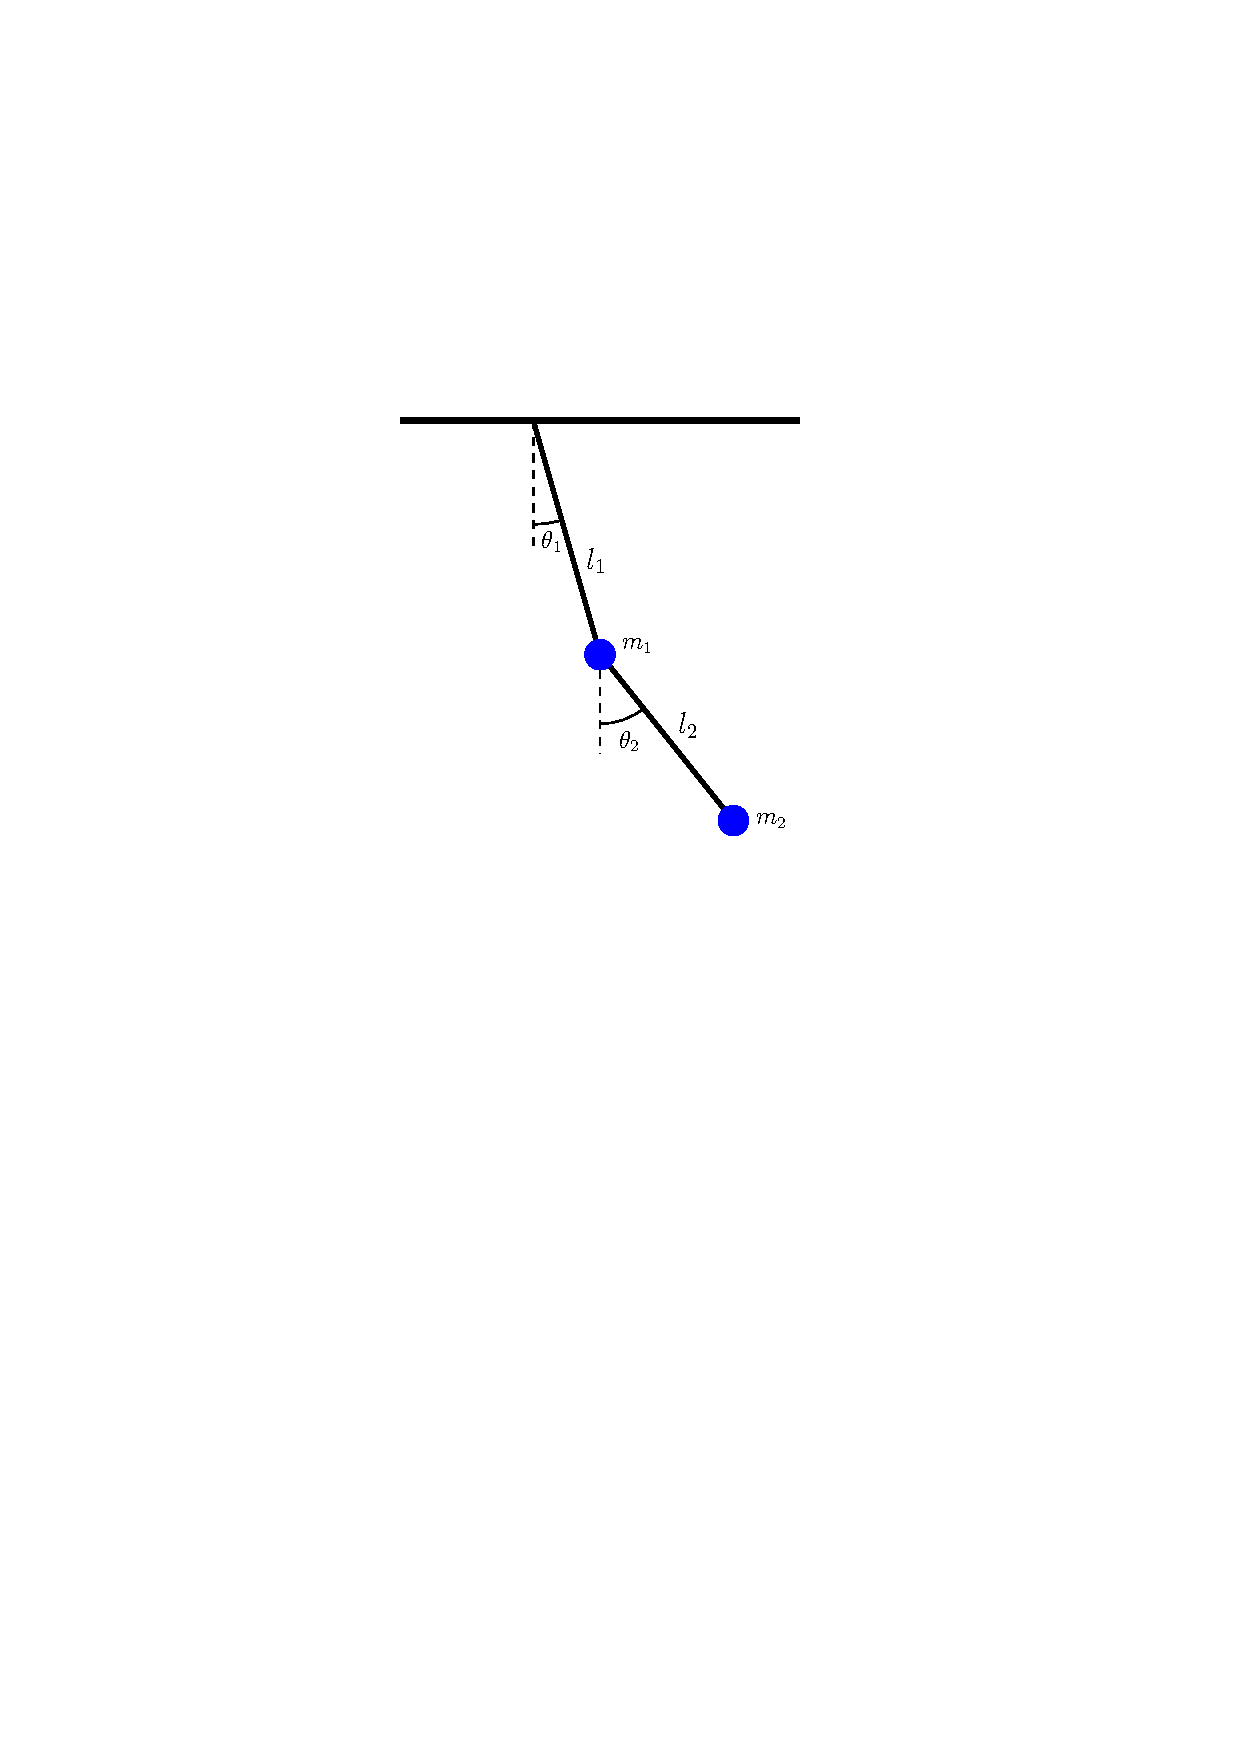
\includegraphics[width=0.45\textwidth]{pic/double pendulum.pdf}
        \caption{Double Pendulum}
        \label{double pendulum}
    \end{figure}
    为方便阅读, 本例中使用黑体字母表示向量.

    {\bf 牛顿力学:} 以双摆的悬挂点为原点, 用 $ \mathbf{r} $ 来表示小球的坐标, 则 
    \begin{align*}
        \mathbf{r}_1 &= l_1(\sin\theta_1,\cos\theta_1),\\
        \dot{\mathbf{r}}_1 &= l_1\dot{\theta}_1(\cos\theta_1,-\sin\theta_1),\\ 
        \ddot{\mathbf{r}}_1 &= l_1\ddot{\theta}_1(\cos\theta_1,-\sin\theta_1)-l_1\dot{\theta}_1^2(\sin\theta_1,\cos\theta_1),\\[2ex]
        \mathbf{r}_2 &= \mathbf{r}_1+l_2(\sin\theta_2,\cos\theta_2),\\
        \dot{\mathbf{r}}_2 &= \dot{\mathbf{r}}_1+l_2\dot{\theta}_2(\cos\theta_2,-\sin\theta_2),\\ 
        \ddot{\mathbf{r}}_2 &= \ddot{\mathbf{r}}_1+l_2\ddot{\theta}_2(\cos\theta_2,-\sin\theta_2)-l_2\dot{\theta}_2^2(\sin\theta_2,\cos\theta_2).
    \end{align*}

    设两个杆上的张力大小分别为 $ T_1 $ 和 $ T_2 $, 则两小球所受的力分别为
    \begin{align*}
        \mathbf{F}_1 &= T_1\frac{-\mathbf{r}_1}{|\mathbf{r}_1|}+T_2\frac{\mathbf{r}_2-\mathbf{r}_1}{|\mathbf{r}_2-\mathbf{r}_1|}+m_1\mathbf{g}=-\frac{T_1}{l_1}\mathbf{r}_1+\frac{T_2}{l_2}(\mathbf{r}_2-\mathbf{r}_1)+m_1\mathbf{g},\\ 
        \mathbf{F}_2 &= T_2\frac{-(\mathbf{r}_2-\mathbf{r}_1)}{|\mathbf{r}_2-\mathbf{r}_1|}+m_2\mathbf{g}=-\frac{T_2}{l_2}(\mathbf{r}_2-\mathbf{r}_1)+m_2\mathbf{g},
    \end{align*}
    带入牛顿定律 $ \mathbf{F}=m\ddot{\mathbf{r}} $ 得到两个方程
    \begin{align*}
        m_1\ddot{\mathbf{r}} &= -\frac{T_1}{l_1}\mathbf{r}_1+\frac{T_2}{l_2}(\mathbf{r}_2-\mathbf{r}_1)+m_1\mathbf{g},\\ 
        m_2\ddot{\mathbf{r}} &= -\frac{T_2}{l_2}(\mathbf{r}_2-\mathbf{r}_1)+m_2\mathbf{g},
    \end{align*}
    按照坐标分量写出来是四个微分方程
    \begin{align*}
        m_1l_1\left( \ddot{\theta}_1\cos\theta_1-\dot{\theta}_1^2\sin\theta_1 \right) &= -T_1\sin\theta_1+T_2\sin\theta_2,\\ 
        -m_1l_1\left( \ddot{\theta}_1\sin\theta_1+\dot{\theta}_1^2\cos\theta_1 \right) &=-T_1\cos\theta_1+T_2\cos\theta_2+m_1g,
    \end{align*}
    \vspace{-1.2cm}
    \begin{align*}
        m_2\left( l_1\ddot{\theta}_1\cos\theta_1-l_1\dot{\theta}_1^2\sin\theta_1+l_2\ddot{\theta}_2\cos\theta_1-l_2\dot{\theta}_2^2\sin\theta_2 \right) &= -T_2\sin\theta_2,\\ 
        -m_2\left( l_1\ddot{\theta}_1\sin\theta_1+l_1\dot{\theta}_1^2\cos\theta_1+l_2\ddot{\theta}_2\sin\theta_1+l_2\dot{\theta}_2^2\cos\theta_2 \right) &= -T_2\cos\theta_2+m_2g,
    \end{align*}
    其中有四个变量 $ \theta_1,\theta_2,T_1,T_2 $.

    分别对前两个和后两个方程以三角函数为系数做线性组合, 可将方程组转化为
    \begin{align*}
        l_1\ddot{\theta}_1 &= \frac{T_2}{m_1}\sin(\theta_2-\theta_1)-g\sin\theta_1,\\
        l_1\dot{\theta}_1^2 &= \frac{T_1}{m_1}-\frac{T_2}{m_1}\cos(\theta_2-\theta_1)-g\cos\theta_1,
    \end{align*}
    \vspace{-1.1cm}
    \begin{align*}
        l_1\ddot{\theta}_1\cos(\theta_2-\theta_1)+l_1\dot{\theta}_1^2\sin(\theta_2-\theta_1)+l_2\ddot{\theta}_2 &= -g\sin\theta_2,\\ 
        -l_1\ddot{\theta}_1\sin(\theta_2-\theta_1)+l_1\dot{\theta}_1^2\cos(\theta_2-\theta_1)+l_2\dot{\theta}_2 &= \frac{T_2}{m_2}-g\cos\theta_2.
    \end{align*}
    关注方程左侧, 在后两个方程中减去前两个方程的成分得
    \begin{align*}
        l_2\ddot{\theta}_2 &= -g\sin\theta_2-\left[ \frac{T_2}{m_1}\sin(\theta_2-\theta_1)-g\sin\theta_1 \right]\cos(\theta_2-\theta_1)\\ 
        &\phantom{=}\;-\left[ \frac{T_1}{m_1}-\frac{T_2}{m_1}\cos(\theta_2-\theta_1)-g\cos\theta_1 \right]\sin(\theta_2-\theta_1)\\ 
        &=-\frac{T_1}{m_1}\sin(\theta_2-\theta_1),
    \end{align*}
    \begin{align*}
        l_2\dot{\theta}_2 &= \frac{T_2}{m_2}-g\cos\theta_2 +\left[ \frac{T_2}{m_1}\sin(\theta_2-\theta_1)-g\sin\theta_1 \right]\sin(\theta_2-\theta_1)\\ 
        &\phantom{=}\;-\left[ \frac{T_1}{m_1}-\frac{T_2}{m_1}\cos(\theta_2-\theta_1)-g\cos\theta_1 \right]\cos(\theta_2-\theta_1)\\ 
        &=\frac{T_2}{m_2}+\frac{T_2}{m_1}-\frac{T_1}{m_1}\cos(\theta_2-\theta_1).
    \end{align*}
    现可将方程组改写为
    \begin{align*}
        l_1\ddot{\theta}_1 &= \frac{T_2}{m_1}\sin(\theta_2-\theta_1)-g\sin\theta_1,\\
        l_1\dot{\theta}_1^2 &= \frac{T_1}{m_1}-\frac{T_2}{m_1}\cos(\theta_2-\theta_1)-g\cos\theta_1,\\ 
        l_2\ddot{\theta}_2 &= -\frac{T_1}{m_1}\sin(\theta_2-\theta_1),\\ 
        l_2\dot{\theta}_2^2 &= \frac{T_2}{m_2}+\frac{T_2}{m_1}-\frac{T_1}{m_1}\cos(\theta_2-\theta_1).
    \end{align*}
    根据第一个和第三个方程, 可以用 $ \theta_1,\theta_2 $ 来表示 $ T_1,T_2 $:
    \begin{align*}
        T_1 &= -m_1\frac{l_2\ddot{\theta}_2}{\sin(\theta_2-\theta_1)},\\ 
        T_2 &= m_1\frac{l_1\ddot{\theta}_1+g\sin\theta_1}{\sin(\theta_2-\theta_1)},
    \end{align*}
    将其带入另外两个方程就得到了双摆的运动方程
    \begin{align*}
        -l_1\dot{\theta}_1^2\sin(\theta_2-\theta_1) &= l_2\ddot{\theta}_2+l_1\ddot{\theta}_1\cos(\theta_2-\theta_1)+g\sin\theta_2\\ 
        l_2\dot{\theta}_2^2\sin(\theta_2-\theta_1) &= \left( \frac{m_1}{m_2}+1 \right)\left( l_1\ddot{\theta}_1+g\sin\theta_1 \right)+l_2\ddot{\theta}_2\cos(\theta_2-\theta_1).
    \end{align*}

    {\bf 拉格朗日力学:} 首先在广义坐标 $ \theta_1,\theta_2 $ 下写出动能和势能
    \begin{align*}
        T &= \frac{1}{2}m_1\dot{\mathbf{r}}_1^2+\frac{1}{2}m_2\dot{\mathbf{r}}_2^2\\ 
        &= \frac{1}{2}m_1l_1^2\dot{\theta}_1^2+\frac{1}{2}m_2\left[ l_1^2\dot{\theta}_1^2+l_2^2\dot{\theta}_2^2+2l_1l_2\dot{\theta}_1\dot{\theta}_2\cos(\theta_2-\theta_1) \right]\\ 
        &= \frac{1}{2}(m_1+m_2)l_1^2\dot{\theta}_1^2+\frac{1}{2}m_2l_2^2\dot{\theta}_2^2+m_2l_1l_2\dot{\theta}_1\dot{\theta}_2\cos(\theta_2-\theta_1),\\
        V &= -m_1gy_1-m_2gy_2 \\ 
        &= -m_1gl_1\cos\theta_1-m_2g(l_1\cos\theta_1+l_2\cos\theta_2)\\ 
        &= -(m_1+m_2)gl_1\cos\theta_1-m_2gl_2\cos\theta_2,
    \end{align*}
    其中 $ y_1,y_2 $ 表示两小球到悬挂点的纵向距离, 于是拉格朗日量为
    \begin{align*}
        L &= T-V\\ 
        &= \frac{1}{2}(m_1+m_2)l_1^2\dot{\theta}_1^2+\frac{1}{2}m_2l_2^2\dot{\theta}_2^2+m_2l_1l_2\dot{\theta}_1\dot{\theta}_2\cos(\theta_2-\theta_1)\\ 
        &\phantom{=}\;+(m_1+m_2)gl_1\cos\theta_1+m_2gl_2\cos\theta_2.
    \end{align*}

    计算关于 $ \theta_1 $ 的拉格朗日方程中的项:
    \begin{align*}
        \frac{\partial L}{\partial\dot{\theta}_1} &= (m_1+m_2)l_1^2\dot{\theta}_1+m_2l_1l_2\dot{\theta}_2\cos(\theta_2-\theta_1),\\ 
        \frac{\mathrm{d}}{\mathrm{d}t}\frac{\partial L}{\partial\dot{\theta}_1} &= (m_1+m_2)l_1^2\ddot{\theta}_1+m_2l_1l_2\ddot{\theta}_2\cos(\theta_2-\theta_1)\\ 
        &\phantom{=}\;-m_2l_1l_2\dot{\theta}_2^2\sin(\theta_2-\theta_1)+m_2l_1l_2\dot{\theta}_1\dot{\theta}_2\sin(\theta_2-\theta_1),\\ 
        \frac{\partial L}{\partial\theta_1} &= m_2l_1l_2\dot{\theta}_1\dot{\theta}_2\sin(\theta_2-\theta_1)-(m_1+m_2)gl_1\sin\theta_1,
    \end{align*}
    写出关于 $ \theta_1 $ 的拉格朗日方程:
    \begin{align*}
        0 &= \frac{\mathrm{d}}{\mathrm{d}t}\frac{\partial L}{\partial\dot{\theta}_1}-\frac{\partial L}{\partial\theta_1}\\ 
        &= (m_1+m_2)l_1^2\ddot{\theta}_1+m_2l_1l_2\ddot{\theta}_2\cos(\theta_2-\theta_1)\\ 
        &\phantom{=}\;-m_2l_1l_2\dot{\theta}_2^2\sin(\theta_2-\theta_1)+(m_1+m_2)gl_1\sin\theta_1.
    \end{align*}
    计算关于 $ \theta_2 $ 的拉格朗日方程中的项:
    \begin{align*}
        \frac{\partial L}{\partial\dot{\theta_2}} &= m_2l_2^2\dot{\theta}_2+m_2l_1l_2\dot{\theta}_1\cos(\theta_2-\theta_1),\\ 
        \frac{\mathrm{d}}{\mathrm{d}t}\frac{\partial L}{\partial\dot{\theta}_2} &= m_2l_2^2\ddot{\theta}_2+m_2l_1l_2\ddot{\theta}_1\cos(\theta_2-\theta_1)\\ 
        &\phantom{=}\;+m_2l_1l_2\dot{\theta}_1^2\sin(\theta_2-\theta_1)-m_2l_1l_2\dot{\theta}_1\dot{\theta}_2\sin(\theta_2-\theta_1),\\ 
        \frac{\partial L}{\partial\theta_2} &= -m_2l_1l_2\dot{\theta}_1\dot{\theta}_2\sin(\theta_2-\theta_1)-m_2gl_2\sin\theta_2,
    \end{align*}
    写出关于 $ \theta_2 $ 的拉格朗日方程:
    \begin{align*}
        0 &= \frac{\mathrm{d}}{\mathrm{d}t}\frac{\partial L}{\partial\dot{\theta_2}}-\frac{\partial L}{\partial\theta_2}\\ 
        &= m_2l_2^2\ddot{\theta}_2+m_2l_1l_2\ddot{\theta}_1\cos(\theta_2-\theta_1)+m_2l_1l_2\dot{\theta}_1^2\sin(\theta_2-\theta_1)+m_2gl_2\sin\theta_2.
    \end{align*}

    这两个拉格朗日方程正是我们前面用牛顿定律推出的运动方程!
\end{example}
虽然两种方法得到了同样的结果, 但使用牛顿力学处理该问题时, 需要用到各种数学技巧, 处理起来也比较麻烦. 在使用拉格朗日力学时, 只需要按部就班地计算就能得到所需的答案.